
\chapter{Introduction}
Making an autonomous robot has been the goal of scientists and engineers for years. This
is a difficult task which includes many disciplines, and has up to date, not been solved in
a general way. Robots which can reason and take own decisions based on how it senses the
environment would greatly simplify our lives in many ways. Many tasks could be completely
outsourced to autonomous robots which do not tier, and is expendable. This means that it
can go places that a human could not. In short this can be summarized into the three Ds,
namely \emph{dull, dirty} and \emph{dangerous} work. Imagine an autonomous robot going
into an earthquake area, mapping out dangerous spots, and where injured people are,
before medical personnel enter the area. Or a robot mapping and inspecting the vast sewer
network of a large city, searching for weak spots and clogged pipes which obstruct the
sewer flow. Or robots crawling the pipelines carrying water, oil or gas to detect leaks
which will cause catastrophic events if not tended to. All of these examples are important work which
is dangerous, dirty or dull, or all three at once.

The problem when a robot is going into an unknown area and mapping the surroundings using
a pack of sensors is formalized into something called \emph{SLAM}, short for
\emph{Simultaneous Localization and Mapping}.
This is a problem that has been thoroughly researched, and has been tried with numerous sensor types
and many solutions are proposed. Some are best in structured environments, like office
landscapes and industrial areas, while other will preform better in more sparse areas with
less landmarks and recognizable features. 

In our global world, the transport of resources, like oil, gas and water are of great importance. Much of this
transport is done using pipelines. There are literally millions of kilometres with pipelines around
the world. Some of these can be inspected from the outside, but most of them are on the
sea floor or under ground and does not allow for outside inspections. 
The pipelines need regular inspections to ensure that the pipeline is intact
and undamaged. Also sewers, as mentioned above, need inspections to keep a satisfactory
standard. Some of the pipes are considered accessible by humans, i.e. diameter over 80 cm,
but most are smaller than this, and uses various inspection devices feeding video to a human
operator that must detect, record, and classify the damages. This is tedious work which
can be automated using robots. \cite{MAKRO-project}

One such robot suitable for pipe inspection might be the \emph{Pipe Inspection Konda}
(PIKo) developed by SINTEF. This is a snake like robot, consisting of a series of identical
modules interconnected by two degrees of freedom active joints. On each module there is a
set of four wheels, two near the ground and two on the top of the modules. For
horizontal motion it uses these wheels and a train like motion to propel itself forward. Since the joints 
connecting the modules have two degrees of freedom, the robot is capable of traversing vertical pipes
as well. This is achieved by spanning the robot inside the pipe alternately and pushing the wheels towards
the pipe walls to gain enough friction for the robot to motion vertically. \cite{piko}

This report will outline a possible navigation system for PIKo. This include the eyes and
ears, the reasoning needed to interpret the senses, together with recollection of the
areas and the decision making on what to do next. Making the robot do this all by it self
is a tremendous task and has up to date not been solved for the general environment.
\begin{figure}[htbp]
    \centering
    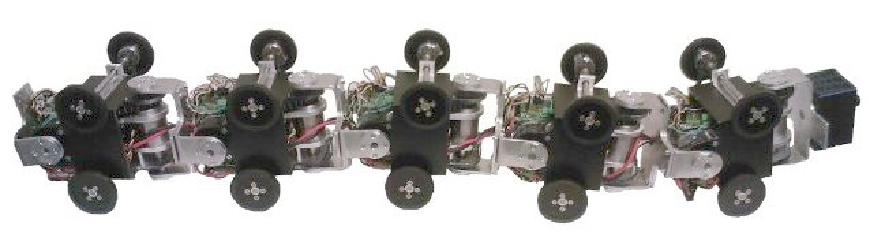
\includegraphics[width=0.8\textwidth]{pics/piko}
    \caption[The Pipe Inspection Konda]{The Pipe Inspection Konda. \url{www.sintef.no}}
    \label{chap1:fig-piko}
\end{figure}

Some of the key challenges when designing such a navigation system are the difficulties
with keeping track of where the robot is, and more importantly where it has been. This is
difficult in a pipe environment because it does not allow for a redundant positioning
system for global position estimation, such as GPS. The robot is then limited to using
either some kind of odometry or determination and tracking of landmarks in the environment, 
or both. The measurement noise will become an important factor when making the map,
because only small errors in the position or orientation will over time give large error
in the map when accumulated over time. \cite{thrun}

When the robot know where it is, it must take the decision on where it should go next. If
there is something blocking the way, it needs to handle these cases in some way.
Unfortunately, the world is not ideal as the usual lab environments and what to expect is
difficult to foresee. 
This calls for a robust system which can handle the situations that can
occur in the given mission environments. 

The report will define and select sensors applicable for a pipe inspection mission
preformed by the PIKo robot platform. The benefits and drawbacks of the different sensors
need to be assessed in detail. Next, the sensor data must be stored and interpreted in some
way, and important features that identify the position in the environment must be selected. 
This calls for processing of sensor data and an intelligent selection of the features that
will describe the environment in the best way. This is known as segmenting a data set.
When the dataset is divided into known geometric features, the estimation of the
parameters of these features can be done. 

PIKo is autonomous platform, and the computational abilities and memory available
are limited. The space available for the map representation is limited.
A map representation with little pre processing takes up much memory, while a
representation which processes the sensor output and estimates features need less space in
memory if the features are recognized by the system. 


\section{Assumptions}
As said above, this is a tremendous task to overcome in the time frame of this project. To
simplify and limit the task some assumptions are taken and summarized below. 
\begin{itemize}
    \item Only planar motion is assumed, even though the implementation platform is
    capable of vertical motion. 
    \item The environment which the robot will operate is structured. Most pipe
    environments are heavily structured. This allows for good prediction on what the robot
    might face in the mission. A good database can be created for what it will encounter. 
\end{itemize}

\section{Demands}
The complete navigation system for a pipe inspection robot should meet the following
demands and qualities. 
\begin{itemize}
    \item Robustness. The system should be robust and able to take the right decisions
    even when the sensors do not give good readings, at least for a limited time.
    \item Real-time system with limited computational abilities. The system is embedded
    and the processor power and memory available are limited. The algorithms should be
    efficient and the sensor data should be treated and stored in a memory efficient way. 
    \item Simplicity. Make thing as simple as possible but not simpler, a great scientist
    once said. This might help to keep the complexity of the system down. 
    \item Consistency. When faced with the same challenge over and over, the robot should
    take the same decision, over and over, because it will be the best one. The robots
    actions should be deterministic. 
    \item Modularity. The navigation system should be designed in a modular way, to allow
    for easy insertion of new features and functionality. 
\end{itemize}


\section{Structure of the Report}
The report is presented in the following way. Chapter \ref{chap2} give a thorough
introduction to the concepts needed to understand this report. It will address different
range finding techniques, and different sensor concepts will be introduced with advantages
and disadvantages of the concepts. Stereo imaging will be discussed in detail, from the
aspect of camera calibration and epipolar geometry to rectification of the captured images and
reprojection of the extracted disparity images. The most used map data representations will be
introduced and explained, also feature extraction and model fitting in Section
\ref{chap2:sec-representations} and \ref{chap2:sec-feature-extraction}. At last, a survey
of the different pipe inspection robots currently under research is included in Section
\ref{chap2:sec-state-of-the-art}.

Chapter \ref{chap3} concerns the selection of sensors appropriate for the application, and
calibration of those sensors. The lens distortion parameters and intrinsic parameters of the
sensors will be estimated and calibrated. 

A representation of the world will be proposed in Chapter \ref{chap5} together with how the sensor
outputs are interpreted.

Chapter \ref{chap6} and \ref{chap7} will deal with implementation and testing of the
proposed system, while Chapter \ref{chap8} will evaluate how the proposed system preformed
on the tests. The last chapter will give the main conclusions and propose further topics
for research. 
